
\begin{frame}[fragile]{Datasets}
\framesubtitle{Explaining the data}
\begin{columns}
\begin{column}{0.6\textwidth}

The data used to train the prediction models come from studies by \emph{The Cancer Genome Atlas Program} (TCGA) and \emph{Oregon Health and Science University} (OHSU) \cite{Genomic-2013, Nature-2018}. Each dataset contains three subsets with data collected from the same patients.

\begin{itemize}
\item Clinical information (CLIN)
\item Gene mutation data (MUT);
\item Gene expression data (EXP).
\end{itemize}
\end{column}


\begin{column}{0.4\textwidth}

\begin{table}[!htb]
    \centering
    \begin{tabular}{c|c|c|}
    
    \cline{2-3}
    &  \textbf{TCGA} & \textbf{OHSU} \\ \hline

    \multicolumn{1}{|l|}{Samples} & 200  &  672 \\ \hline
    \multicolumn{1}{|l|}{Patients}  & 200 & 562 \\ \hline
    \multicolumn{1}{|l|}{\emph{CLIN}} & 31  & 97 \\ \hline
    \multicolumn{1}{|l|}{\emph{MUT}} & 25,000 &  606 \\ \hline
   \multicolumn{1}{|l|}{\emph{EXP}} & 25,000 & 22,825 \\ \hline
    \end{tabular}
    \caption{Number of samples and features present in the datasets.}
\end{table}

\end{column}
\end{columns}

\end{frame}



\begin{frame}{Data cleaning and preprocessing}
\framesubtitle{Explaining the data}

Since the datasets are from different sources, they must be processed to ensure consistency.  With the support of specialists, we removed the following spurious data:

\begin{columns}
    \begin{column}{0.5\textwidth}
    \begin{itemize}
     \item Samples not considered as adult AML. The age of the patient must not be less than 18 years;
    \item Samples in which the percentage of blasts in the bone marrow were lower than 20\%;
    \item Duplicate samples;
    \end{itemize}
    \end{column}

    \begin{column}{0.5\textwidth}
    \begin{itemize}
        \item Samples without information on survival elapsed time after treatment (\textit{Overall Status Survival});
        \item Samples and features of patients in only one of two databases;
        \item Features with all values empty.
    \end{itemize}
\end{column}    
\end{columns}
    
\end{frame}


\begin{frame}{Data Cleaning and Preprocessing}
\framesubtitle{Explaining the data}

Additionally, the following steps were taken in the preprocessing stage:

\begin{itemize}
    \item Automatically filling empty values in clinical data features (CLIN) with the 3-NN method;
    \item Kept only the samples in which all the variables are compatible, observing data related to the exams and treatment received by the patients
    \item Cytogenetic information was normalized and grouped by AML specialists.
    \item Treatment information was also grouped  into four categories according to the intensity of each therapy: \emph{Target therapy}, \emph{Regular therapy}, \emph{Low-Intensity therapy} and \emph{High-Intensity therapy}.
\end{itemize}

    %Table with number of remaining samples and features 
    
\end{frame}

%INCLUDE A GRAPHIC INSTEAD
\begin{frame}{Number of samples}

Of the \emph{872} initial samples in the two databases, \emph{272} were kept at the end of the preprocessing and data-cleaning processes. 

\begin{columns}

    \begin{column}{0.4\textwidth}
    \begin{center}
        \begin{figure}
            \centering
            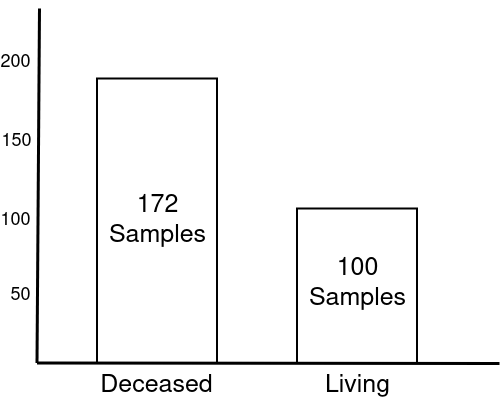
\includegraphics[width=0.7\textwidth]{beamerthemesrc/figs/class_distribution.png}
            \caption{Class distributions after preprocessing}
            \label{fig:classdist}
        \end{figure}
    \end{center}
    \end{column}
    
    \begin{column}{0.4\textwidth}

    \begin{table}[!htb]
    \centering
    \begin{tabular}{c|c|}
    
    \cline{2-2}
    &  \textbf{Merged datasets} \\ \hline

    \multicolumn{1}{|l|}{Samples} & 272 \\ \hline
    \multicolumn{1}{|l|}{Patients}  & 272 \\ \hline
    \multicolumn{1}{|l|}{\emph{CLIN}} & 11 \\ \hline
    \multicolumn{1}{|l|}{\emph{MUT}} & 281 \\ \hline
   \multicolumn{1}{|l|}{\emph{EXP}} & 14,712 \\ \hline
    \end{tabular}
    \caption{Number of samples and features present in the preprocesed datasets.}
\end{table}


    
    \end{column}
        
    
\end{columns}

\end{frame}



%INCLUDE A GRAPHIC INSTEAD
\begin{frame}{Clinical Features}
\framesubtitle{Feature Selection}
The clinical features were selected by specialists in the data domain according to their relevance for predicting clinical outcomes.

\vspace{0.25cm}
\begin{itemize}
    \item The selected features are:
    \emph{Diagnosis age, Bone marrow blast (\%), Mutation count, PB blast (\%), WBC, Sex, Race, Cytogenetic info, ELN risk classification, Treatment intensity classification,  Overall survival status (class)}.
\end{itemize}
\vspace{0.25cm}

One noticeable highlight is that the patient's age seems to be a good predictor of the outcome. \emph{The older the patient, the lower the chances of survival}. 

\end{frame}



\begin{frame}{Gene Mutation Features}
\framesubtitle{Feature Selection}
\begin{itemize}
    \item The $\chi^2$ statistical method was used to select gene mutation features \cite{Rahman-2019}.
    \item The following hypotheses were defined:
    \begin{itemize}
        \item H0 -- patient survival is independent of gene mutation;
        \item H1 -- both groups are dependent.
    \end{itemize}
    \item Using $p < 0.05$, only two features were selected: \textit{PHF6} and \textit{TP53} gene mutations;

    \begin{block}{}
    \vspace{0.25cm}
    To further investigate the potential of gene mutation data we have enriched the set with well-known genes in the literature and used by the ELN: \textit{FLT3}, \textit{NPM1}, \textit{DNMT3A}, \textit{IDH1}, \textit{IDH2}, \textit{TET2}, \textit{ASXL1}, \textit{RUNX1}, \textit{CEBPA}, \textit{NRAS}, \textit{KRAS}, \textit{SF3B1}, \textit{U2AF1}, \textit{SRSF2} \cite{Lagunas-Rangel-2017, Pimenta-2021, Charrot-2020} \cite{Dohner-2022}.
    \vspace{0.25cm}
\end{block}
   
\end{itemize}
\end{frame}



%\begin{frame}{Gene Mutation Features}
%\framesubtitle{Selected Genes}

%\begin{itemize}
    %\item The \emph{TP53} is considered a controller of genomic stability, mutations of this gene are found in approximately half of cancer patients \cite{kastenhuber-2017-28886379}. In AML patients, although less common, mutations in \emph{TP53} are associated with a poor prognosis~\cite{grob-2022-35108372};
    
    %\item PHF6 is a tumor suppressor gene, and several studies have shown a high mutation frequency in the adverse risk group of AML~\cite{Eisa-2023}. 
%\end{itemize}
    
%\end{frame}


\begin{frame}{Gene Expression Features}
\framesubtitle{Feature Selection}

\begin{itemize}
    \item To select the most relevant features for outcome prediction, we have employed a method similar to Lasso Regression \cite{Tibshirani-1996}: we have trained an SVM model with L1 regularization.
    %\item This method estimates the relevance of the features by assigning a weight coefficient to each of them. When a feature receives a zero coefficient, it is irrelevant enough for the problem the model was trained for. As a consequence, these features are not selected.
    \item The method was trained with all 14,712 gene expression features, from which 22 were selected.
    
    
\end{itemize}
    
\end{frame}


\begin{frame}{Final Selected Features}
The image below resumes the resulting datasets after the steps of cleaning, preprocessing and feature selection.
\framesubtitle{Feature Selection}
    \begin{figure}
        \centering
        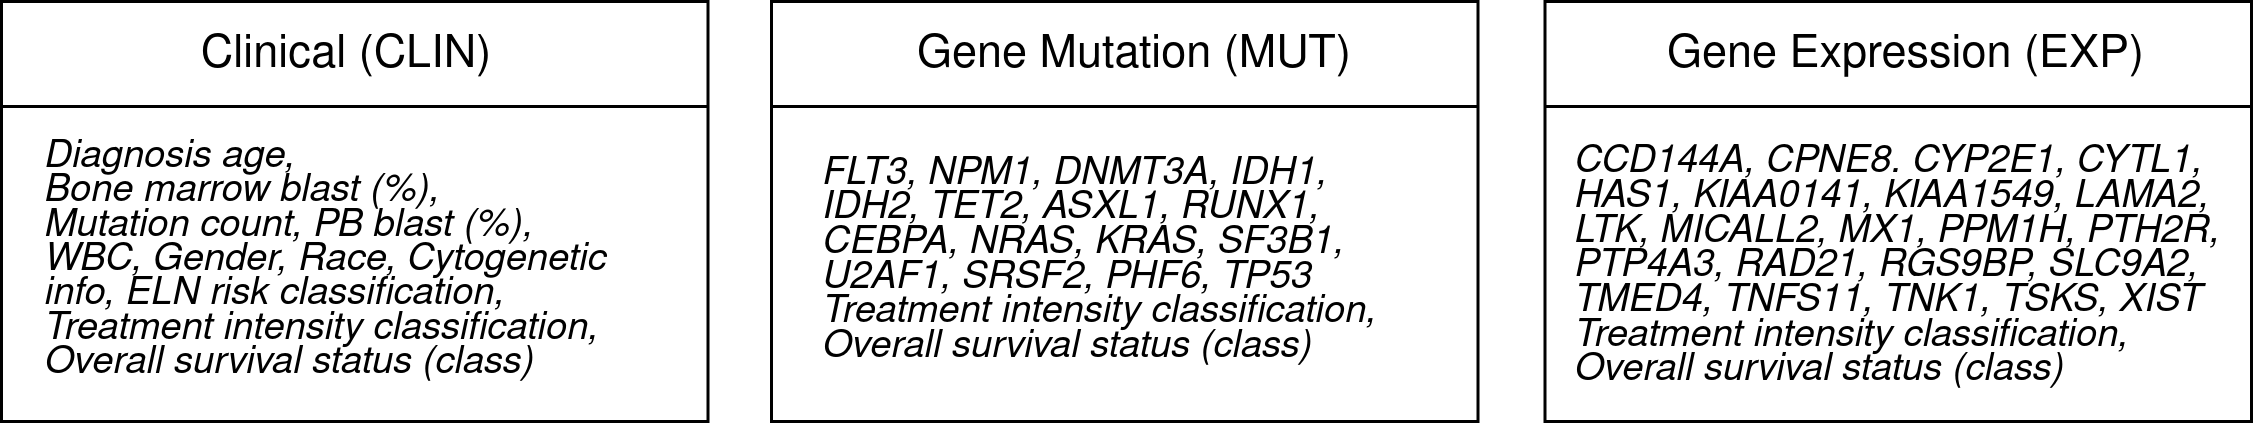
\includegraphics[width=1\textwidth]{beamerthemesrc/figs/selected_features.png}
        \caption{Final features present in the datasets}
        \label{fig:feature_sel}
    \end{figure}
\end{frame}



\begin{frame}{Explainable Boosting Machines}
\framesubtitle{Training the outcome prediction models}

Since interpretability is crucial for machine-learning models in medicine~\cite{Combi-2022}, we have employed the Explainable Boosting Machine (EBM) technique~\cite{Caruana-2015}.


\begin{itemize}
    \item Combines the strengths of boosting techniques with the goal of interpretability;
    \item Incorporates a set of interpretable rules defined by individual input features;
    \item EBM automatically learns the optimal rules and their associated weights to create an ensemble of rule-based models, where the weights reflect the importance of each rule in the overall prediction;
    \item EBM has been applied successfully in various domains, such as predicting medical conditions and other scenarios where interpretability and transparency are paramount~\cite{pmlr-v139-nori21a}.
\end{itemize}

\end{frame}


\begin{frame}{Explainable Boosting Machines}
\framesubtitle{Performance evaluation}

We have used the EBM classification method from the InterpretML library to train the outcome prediction models.

\begin{itemize}
    \item We trained one model per dataset (CLIN, MUT, EXP) and four using all possible combinations of data (CLIN+MUT, CLIN+EXP, MUT+EXP, CLIN+MUT+EXP).
    \item  Performance evaluation was done using holdout \cite{Mitchell-1997}. The data was randomly divided into three parts:  80\% for training the models, 10\%  for model and feature selection, and the remaining 10\% was used to test.
\end{itemize}

To evaluate the models, we calculated the following measures: accuracy, recall (or sensitivity), precision, F1-Score, and the Area Under the ROC Curve (AUC).
    
\end{frame}